%%%%%%%%%%%%%%%%%%%%%%%%%%%%%%%%%%%%%%%%%%%%%%
%%% This is a script written for iAstro (http://iastro.lamost.org).
%%% Author: MA[family] Lei
%%% Created: 2012-02-10
%%% CC BY-NC-SA
%%%%%%%%%%%%%%%%%%%%%%%%%%%%%%%%%%%%%%%%%%%%%%

\documentclass{article}
\usepackage{tikz,times}
\usepackage[paperwidth=1000pt,paperheight=1000pt,left=20pt,top=20pt]{geometry}

\usepackage{pifont}



\usetikzlibrary{mindmap,backgrounds}
\pgfdeclarelayer{background}
\pgfdeclarelayer{foreground}
\pgfsetlayers{background,main,foreground}


\pagestyle{empty}

\begin{document}

{\centering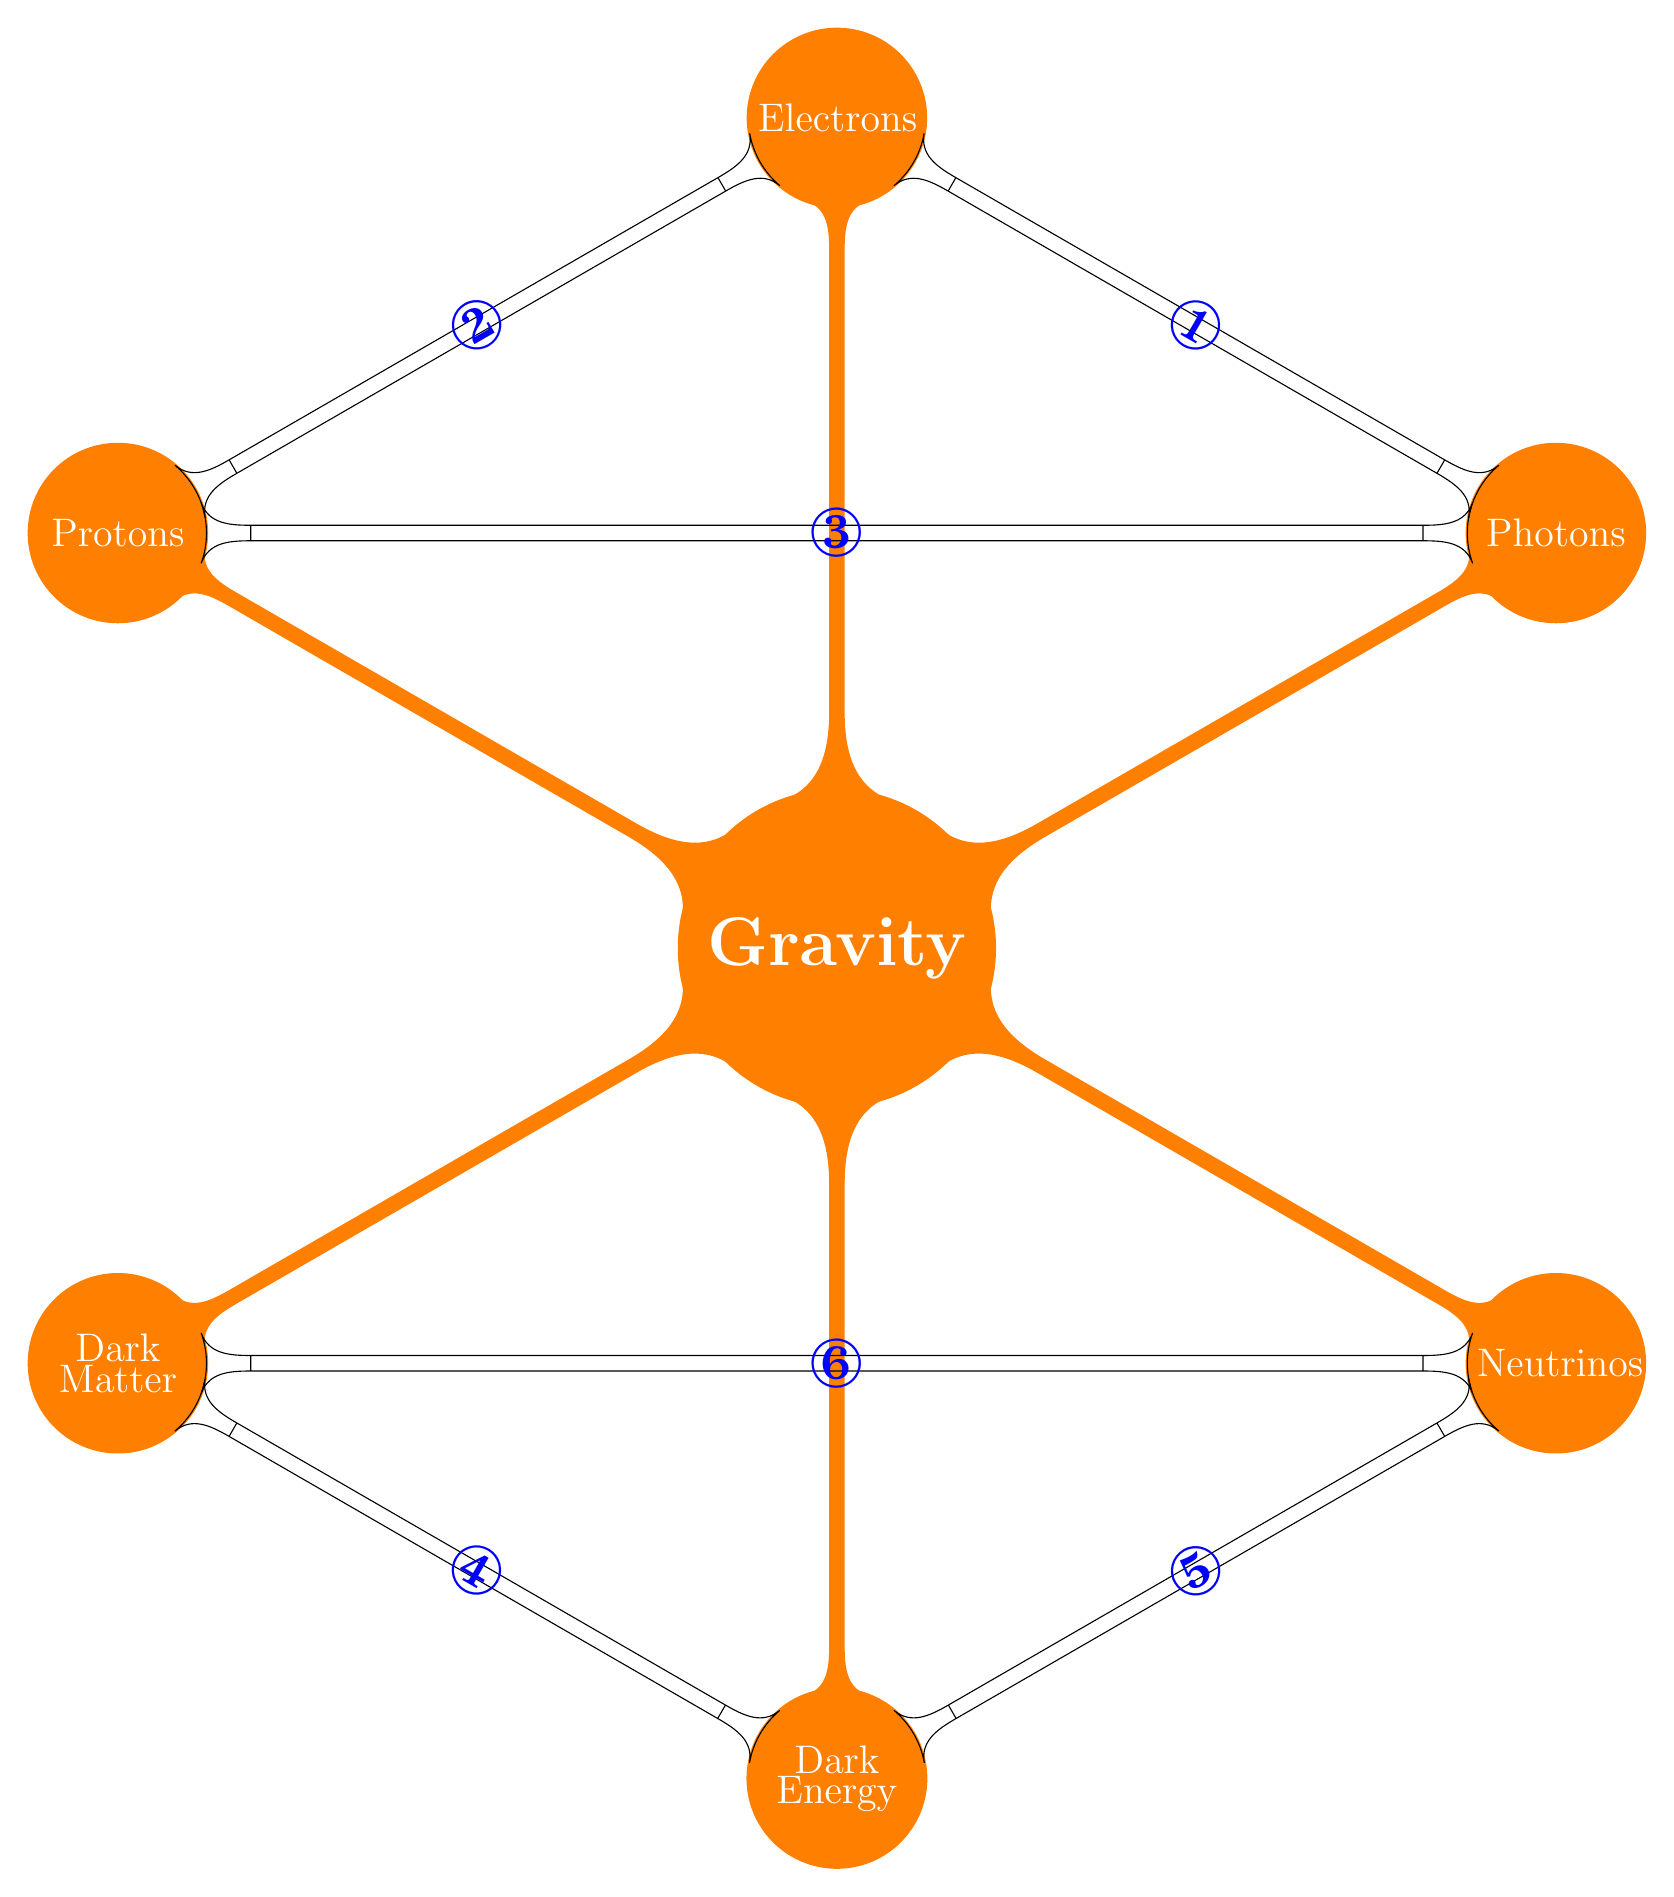
\begin{tikzpicture}[mindmap,
  level 1 concept/.append style={level distance=300,sibling angle=60},
  extra concept/.append style={color=blue!50,text=black}]

  % Gravity is the center of everything, so is that weird that such a universal thing exist.

  \begin{scope}[mindmap, concept color=orange, text=white]
    \node [concept] {\bf \Huge Gravity}[clockwise from=-30] 
      child {node [concept] (neu) {\Large  Neutrinos}}
      child {node [concept] (de) {\Large Dark Energy}}
      child {node [concept] (dm) {\Large Dark Matter}}
      child {node [concept] (pr) {\Large Protons}}
      child {node [concept] (ele) {\Large Electrons}}
      child {node [concept] (ph) {\Large Photons}};
  \end{scope}





  \begin{pgfonlayer}{foreground}
    \draw [circle connection bar]
      (ph) edge node [sloped] {\Huge\color{blue} \ding{172}} (ele)
      (ele) edge node [sloped] {\Huge\color{blue}\ding{173}} (pr)
      (pr) edge node [sloped] {\Huge\color{blue}\ding{174}} (ph)
      (dm) edge node [sloped] {\Huge\color{blue}\ding{175}} (de)
      (de) edge node [sloped] {\Huge \color{blue}\ding{176}} (neu)
      (dm) edge node [sloped] {\Huge\color{blue} \ding{177}} (neu);
  \end{pgfonlayer}
\end{tikzpicture}

}

 {\color{gray}\huge\bf{~ \{References\}\footnote{I just leave out other particles and the interaction between neutrinos and electrons. This is not a figure about all kinds of fields but a figure about what is concerned in cosmology.}
}}
\begin{quote}\Large\color{gray}
\begin{description}
\item[\color{green}\ding{182}]
Compton Scattering before Recombination.
\item[\color{green}\ding{183}]
Coulomb Scattering/Thomson Scattering.
\item[\color{green}\ding{184}]
Compton Scattering before Recombination.
\item[\color{green}\ding{185}]
Possible Interaction.

Related papers are arXiv:hep-th/9408025, arXiv:astro-ph/9908023, arXiv:0804.0232.
\item[\color{green}\ding{186}]
Possible Interaction. 

Related papers are arXiv:0802.1515, arXiv:1106.2161, arXiv:1009.2461, arXiv:1110.2173.
\item[\color{green}\ding{187}]
Weak Interaction.


\end{description}

\end{quote}

\end{document}